Os estudos de caso singulares (Casos 1 e 2) avaliados nessa seção foram propostos por \citeonline{jacobson_computation_1970} e utilizados na validação de um método proposto pelo autor para solução de PCOs singulares. Desde então, vários outros autores \cite{nascentes_resolucao_2012, iasbeck_resolucao_2020} os têm empregado com essa mesma finalidade. % No Apêndice \ref{apd:singulares}, demonstra-se que os estudos de caso em questão são de fato singulares. 

Verifica-se por meio da análise das soluções reportadas por \citeonline{jacobson_computation_1970} (ver as Figuras \ref{fig:singular1:jacobson} e \ref{fig:singular2:jacobson}), que os perfis de controle associados às soluções de cada um dos estudos de caso são descontínuos em $ t \approx 1,5$ s. Assim, espera-se que a presença de descontinuidades nas trajetórias de controle dificulte a resolução desses problemas, principalmente ao se aplicar a colocação pseudo-espectral, uma vez que desaconselha-se o emprego desse tipo de abordagem para a determinação de trajetórias não suaves \cite{becerra_tutorial_2010}. 

\noindent	
\begin{minipage}{\textwidth}
	\vspace{\onelineskip}
	\centering
	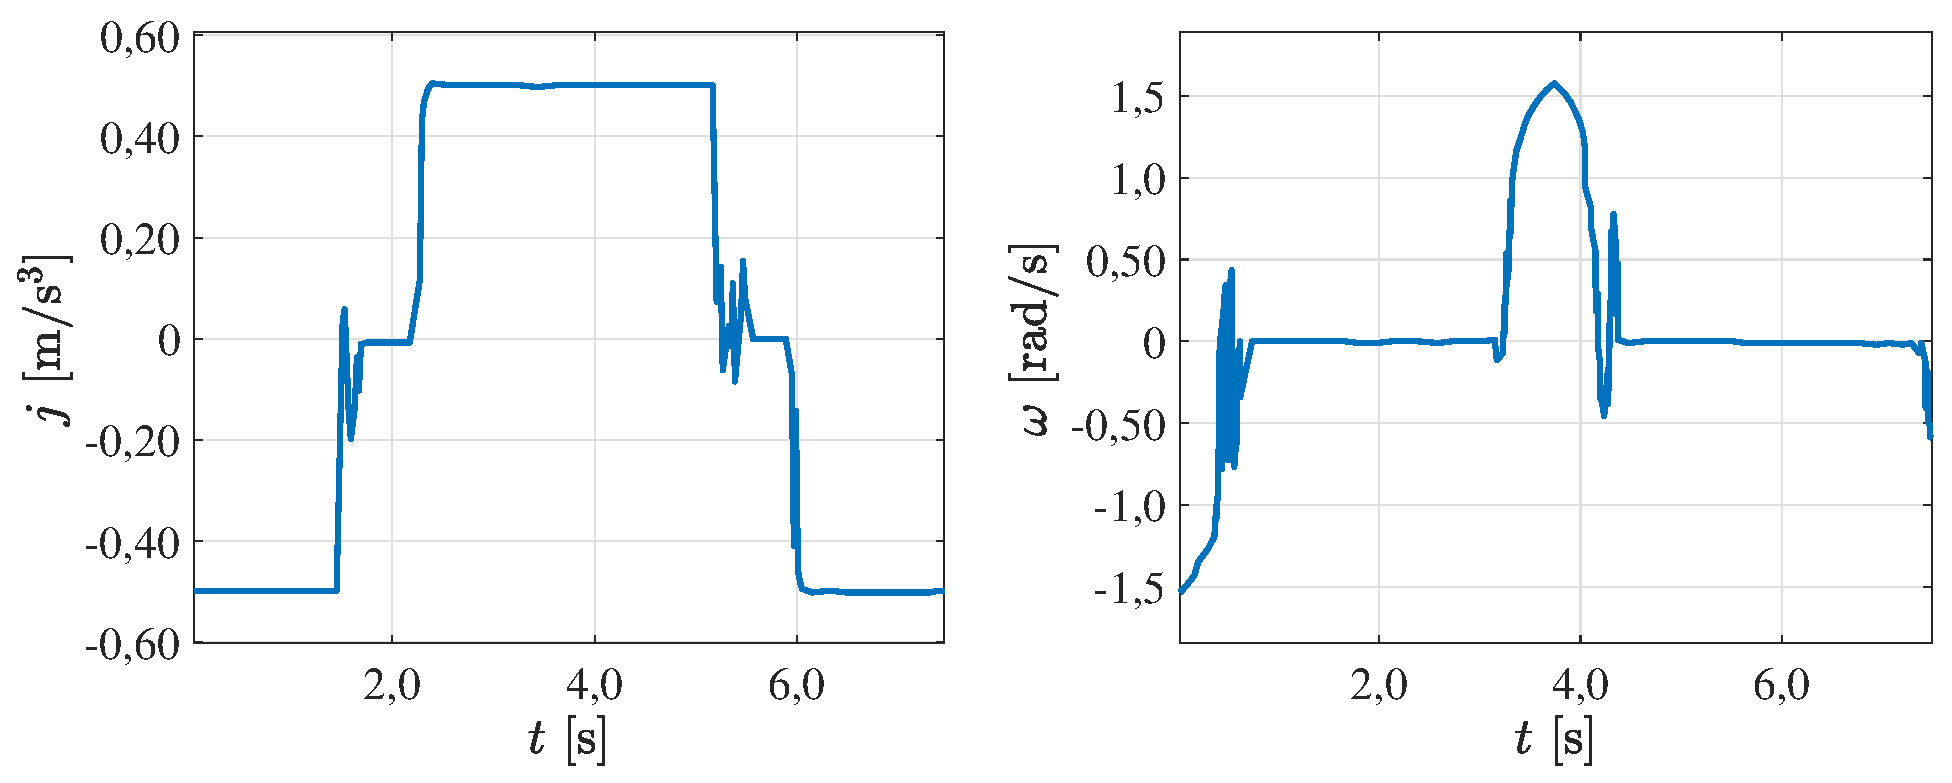
\includegraphics[scale=0.7]{fig/resultados/singular1/obs/original}
	\captionof{figure}[Solução do problema singular 1 reportada na literatura]{Resultado reportado por \citeonline{jacobson_computation_1970} para o estudo de caso descrito na Seção \ref{sec:singular1}.}
	\label{fig:singular1:jacobson}
	\vspace{\onelineskip}
\end{minipage} 

\noindent	
\begin{minipage}{\textwidth}
	\vspace{\onelineskip}
	\centering
	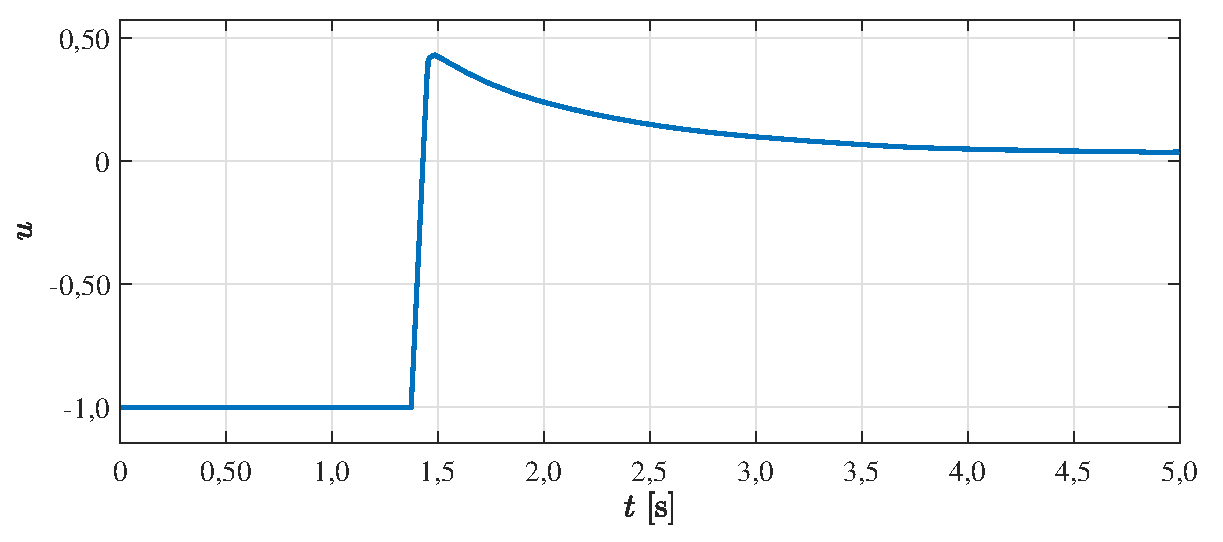
\includegraphics[scale=0.7]{fig/resultados/singular2/obs/original}
	\captionof{figure}[Solução do problema singular 2 reportada na literatura]{Resultado reportado em \citeonline{jacobson_computation_1970} para o estudo de caso descrito na Seção \ref{sec:singular2}.}
	\label{fig:singular2:jacobson}
	\vspace{\onelineskip}
\end{minipage} 